\documentclass[11pt]{article}

\usepackage{amsmath,amssymb,bm,booktabs,graphicx,hyperref}
\usepackage[margin=1in]{geometry}

\title{Trial 001: Numerical-GP Wildfire-Spread Prediction via\\
Universal-Kriging Initialisation and Ensemble Pushforward\\
of the Rothermel Level-Set Operator}
\author{}
\date{}

\newcommand{\bx}{\mathbf{x}}
\newcommand{\bw}{\mathbf{w}}
\newcommand{\GP}{\mathcal{GP}}
\newcommand{\N}{\mathcal{N}}

\begin{document}
\maketitle

\section{Governing Physics}

Let $\phi^{n}(\bx)$ be the level-set field on the grid $\bx=(x,y)$ at time
$t_n=n\,\Delta t$, with $\phi<0$ burned, $\phi>0$ unburned, and the fire front at
$\phi=0$. The simulator (\texttt{simulation.ipynb}) evolves the Rothermel-driven
level set

\begin{equation}
  \label{eq:levelset}
  \phi_t \;=\; \mathcal{N}[\phi]
  \;:=\; -\,R_f(\phi)\,\lvert\nabla\phi\rvert
  \;+\; \nu\,\Delta x\,\nabla^{2}\phi ,
\end{equation}

where $\nu=0.4$ is the (numerical) viscosity coefficient and the $\nu\,\Delta x$
prefactor is taken verbatim from the simulator. The rate of spread $R_f$ is the
Rothermel (1972) imperial form, decomposed (slope $=0$, height field zeroed) as

\begin{equation}
  \label{eq:Rf}
  R_f(\phi) \;=\; R_0\,\bigl(1+\phi_W(\bx)\bigr),
  \qquad
  R_0=\frac{I_R\,\xi}{\rho_b\,\varepsilon_h\,Q_{ig}},
\end{equation}

with reaction intensity $I_R$, propagating-flux ratio $\xi$, ovendry bulk density
$\rho_b$, effective heating number $\varepsilon_h$, and heat of preignition
$Q_{ig}$. The wind factor couples the front \emph{normal}
$\hat{\mathbf n}=\nabla\phi/\lvert\nabla\phi\rvert$ to the midflame wind
$\mathbf{w}$:

\begin{equation}
  \label{eq:windfactor}
  \phi_W(\bx)=C\,U(\bx)^{B}\,(\beta/\beta_{op})^{-E},
  \qquad
  U(\bx)=\max\!\bigl(0,\;\mathbf{w}\cdot\hat{\mathbf n}(\bx)\bigr),
\end{equation}

so $R_f$ is largest where the front normal aligns with the wind (downwind, NE
here) and falls to $R_0$ where $U=0$. The clamp $U\ge 0$ avoids fractional powers
of negatives (simulator behaviour). Eq.~\eqref{eq:windfactor} makes
\eqref{eq:levelset} \emph{nonlinear and non-local in $\nabla\phi$}.

\begin{table}[h]
  \centering
  \caption{Constants and parameters (from \texttt{simulation.ipynb}; see \texttt{gp/UNITS.md}).}
  \label{tab:constants}
  \begin{tabular}{@{}llll@{}}
    \toprule
    Symbol & Value & Units & Description \\
    \midrule
    grid & $200\times200$ & cells & $5\,\mathrm{km}\times5\,\mathrm{km}$ \\
    $\Delta x$ & $82.021$ & ft $(=25$\,m$)$ & grid spacing \\
    $\Delta t$ & $1$ & min & implicit Euler step \\
    $\nu$ & $0.4$ & -- & viscosity coefficient \\
    $\mathbf{w}$ & $(100,100)$ & ft/min & midflame wind ($|\mathbf{w}|=141.4$) \\
    $R_0$ & $3.8065$ & ft/min & base ROS (no wind) \\
    $R_f^{\max}$ & $9.6834$ & ft/min & full-wind ROS ($U=|\mathbf w|$) \\
    $I_R$ & $730.93$ & -- & reaction intensity \\
    $\xi$ & $0.05775$ & -- & propagating-flux ratio \\
    $\rho_b$ & $0.0340$ & -- & ovendry bulk density \\
    $\varepsilon_h$ & $0.96134$ & -- & effective heating number \\
    $Q_{ig}$ & $339.28$ & -- & heat of preignition \\
    $C,\,B$ & $5.42\!\times\!10^{-5},\,2.0712$ & -- & wind-factor constants \\
    $(\beta/\beta_{op})^{-E}$ & $1.0000$ & -- & wind-factor packing term \\
    \bottomrule
  \end{tabular}
\end{table}

\section{Method}

\subsection{Prior placement}

We place the GP prior on the \emph{unknown initial field} $\phi^{0}$ (the only
latent quantity; the operator $\mathcal{N}$ is known). To keep the prior general
and free of any ignition-geometry assumption, we use universal kriging: a generic
low-order trend mean plus a stationary RBF residual,

\begin{equation}
  \label{eq:prior}
  \phi^{0}(\bx)\sim\GP\!\bigl(m_{\bm\beta}(\bx),\;k(\bx,\bx')\bigr),
  \qquad
  m_{\bm\beta}(\bx)=\mathbf{p}(\bx)^{\!\top}\bm\beta,
  \quad
  k(\bx,\bx')=\sigma_f^{2}\,e^{-\lVert\bx-\bx'\rVert^{2}/2\ell^{2}}.
\end{equation}

Here $\mathbf{p}(\bx)=[\,1,u,v,u^{2},v^{2},uv\,]$ with $u=(x-100)/100$,
$v=(y-100)/100$ (normalised by the public domain half-width, not the unknown fire
location). \textbf{The quadratic trend is a smooth bowl; it cannot represent the
square / signed-distance front. All front geometry is supplied by the RBF residual
conditioned on data.} We realise both blocks as one Bayesian linear model with
feature map $\bm\Phi(\bx)=[\,\mathbf{p}(\bx)^{\!\top},\,\mathbf{z}(\bx)^{\!\top}\,]^{\!\top}$,
where the random Fourier features

\begin{equation}
  \label{eq:rff}
  z_j(\bx)=\sqrt{\tfrac{2}{M}}\,\sigma_f\cos(\bm\omega_j^{\!\top}\bx+b_j),
  \quad \bm\omega_j\sim\N(\mathbf{0},\ell^{-2}I),\;\; b_j\sim U[0,2\pi],
\end{equation}
satisfy $\sigma_f^{2}\,\mathbb{E}[\mathbf z(\bx)^{\!\top}\mathbf z(\bx')]\to
k(\bx,\bx')$ as $M\to\infty$. With weight prior
$\bw\sim\N(\mathbf 0,\Lambda)$, $\Lambda=\mathrm{blkdiag}(\tau^{2}I_6,I_M)$ (flat
on the trend, $\tau=10^{3}$), the field is $\phi^{0}(\bx)=\bm\Phi(\bx)^{\!\top}\bw$.

\subsection{Euler discretisation and numerical GP construction}

The embedded time-stepper is forward Euler on \eqref{eq:levelset}
($\Delta t=1$), defining the (nonlinear) Euler map $\mathcal{E}$:

\begin{equation}
  \label{eq:euler}
  \phi^{n}=\mathcal{E}[\phi^{n-1}]
  :=\phi^{n-1}+\Delta t\,\mathcal{N}[\phi^{n-1}]
  =\phi^{n-1}+\Delta t\bigl(-R_f^{\,n-1}\lvert\nabla\phi^{n-1}\rvert
  +\nu\,\Delta x\,\nabla^{2}\phi^{n-1}\bigr).
\end{equation}

Following the Numerical GP construction, linearising $\mathcal{E}$ about the
current mean $m_{n-1}$ gives the Jacobian
$J_{n-1}=I+\Delta t\,\mathcal{N}'[m_{n-1}]$ and the joint multi-output GP for two
consecutive steps,

\begin{equation}
  \label{eq:joint-gp}
  \begin{bmatrix}\phi^{n}\\[2pt]\phi^{n-1}\end{bmatrix}
  \sim\GP\!\left(
  \begin{bmatrix}\mathcal{E}[m_{n-1}]\\[2pt] m_{n-1}\end{bmatrix},\;
  \begin{bmatrix}
    J_{n-1}K_{n-1}J_{n-1}^{\!\top}+Q & J_{n-1}K_{n-1}\\[2pt]
    K_{n-1}J_{n-1}^{\!\top} & K_{n-1}
  \end{bmatrix}\right),
\end{equation}

i.e.\ the cross-covariance is the operator applied to the previous kernel,
$k^{n,n-1}(\bx,\bx')=(J_{n-1}\!\cdot k^{n-1,n-1})(\bx,\bx')$, and the marginal
propagates as $m_n=\mathcal{E}[m_{n-1}]$, $K_n=J_{n-1}K_{n-1}J_{n-1}^{\!\top}+Q$
($Q\succeq 0$ optional process noise; $Q=0$ here).

\paragraph{Computational realisation (ensemble pushforward).}
A dense $K_n\in\mathbb{R}^{40000\times40000}$ is intractable, and the strong
nonlinearity of $\lvert\nabla\phi\rvert$ and \eqref{eq:windfactor} makes a single
Jacobian linearisation lossy. We therefore propagate the covariance by Monte-Carlo
pushforward of the $t=0$ posterior through the \emph{exact} operator
$\mathcal{E}$: draw $N$ posterior samples $\phi^{0}_{s}$, advance each by
\eqref{eq:euler}, and estimate

\begin{equation}
  \label{eq:ensemble}
  m_n\approx\frac1N\sum_{s=1}^{N}\phi^{n}_s,
  \qquad
  K_n\approx\frac1{N-1}\sum_{s=1}^{N}
  (\phi^{n}_s-m_n)(\phi^{n}_s-m_n)^{\!\top},
  \qquad \phi^{n}_s=\mathcal{E}^{\,n}[\phi^{0}_s].
\end{equation}

This is \eqref{eq:joint-gp} without the first-order truncation: the ensemble
carries the GP covariance to every evaluation time and captures curvature/wind
nonlinearity that $J_{n-1}$ alone would drop. We report the diagonal
$\sigma_n(\bx)=\sqrt{\mathrm{diag}\,K_n}$ as predictive uncertainty.

\subsection{Inference from sparse observations}

With observation model $y_i=\phi^{0}(\bx_i)+\eta_i$, $\eta_i\sim\N(0,\sigma_n^2)$,
$i=1\dots50$, the weight posterior is exact Bayesian linear regression,

\begin{equation}
  \label{eq:posterior}
  \bw\mid\mathbf y\sim\N(\bm\mu_w,\Sigma_w),
  \quad
  \Sigma_w=A^{-1},\;\;
  A=\sigma_n^{-2}\bm\Phi_X^{\!\top}\bm\Phi_X+\Lambda^{-1},\;\;
  \bm\mu_w=\sigma_n^{-2}A^{-1}\bm\Phi_X^{\!\top}\mathbf y,
\end{equation}

where $\bm\Phi_X\in\mathbb{R}^{50\times(6+M)}$ stacks the features at the
observation cells. The posterior field mean is $m_0(\bx)=\bm\Phi(\bx)^{\!\top}\bm\mu_w$
and posterior IC draws are $\phi^{0}_s=\bm\Phi\,\bw_s$,
$\bw_s=\bm\mu_w+R^{-\top}\bm\eta_s$ with $A=RR^{\!\top}$, $\bm\eta_s\sim\N(0,I)$.
The lengthscale $\ell$ is selected by maximising the exact-RBF log marginal
likelihood of the \emph{detrended} observations over
$\ell\in\{8,\dots,24\}$ (data-only; no ground truth), giving $\ell=16$ cells.

\subsection{Algorithm}

\begin{enumerate}\itemsep0pt
  \item Sample 50 observation values from $\phi^{0}$ in the central window
        $[50,150)^2$ (seed 42).
  \item Select $\ell$ by detrended marginal likelihood; form the BLR posterior
        \eqref{eq:posterior} from the 50 values only.
  \item Draw $N=128$ posterior initial fields $\phi^{0}_s$.
  \item Advance each $\phi^{0}_s$ by the embedded Euler map \eqref{eq:euler} for
        300 steps, recording $t\in\{50,100,150,200,250,300\}$.
  \item Report ensemble mean \eqref{eq:ensemble} as the prediction and ensemble
        std as uncertainty; compare to the simulator ground truth.
\end{enumerate}

\section{Assumptions and approximations}

\begin{itemize}\itemsep1pt
  \item \textbf{Known operator, faithful re-implementation.} The embedded operator
        \eqref{eq:euler}--\eqref{eq:windfactor} is mathematically identical to the
        simulator's Rothermel level-set Euler step but is a separate
        implementation (no shared function). Consequently forecast error is
        dominated by the \emph{propagated $t=0$ reconstruction error}, reported
        separately from the reconstruction error itself (Sec.~\ref{sec:results}).
  \item \textbf{Universal-kriging mean.} The quadratic trend is a generic smooth
        bowl, not an ignition-shape prior. In the unobserved far field the
        posterior reverts to this trend, which overshoots the true signed
        distance; hence \emph{full-grid} RMSE is dominated by the far field, while
        the fire (which never leaves $[80,140]^2$) is governed by the central
        window.
  \item \textbf{Covariance via ensemble pushforward} \eqref{eq:ensemble}, not a
        dense kernel; first-order term in \eqref{eq:joint-gp} is superseded by the
        exact nonlinear pushforward. RFF ($M=512$) approximates the RBF kernel.
  \item \textbf{No reinitialisation} of $\phi$ on \emph{either} side (symmetric):
        the simulator never redistances, so $\lvert\nabla\phi\rvert$ drifts from 1
        identically in prediction and ground truth.
  \item \textbf{Boundaries ignored} (infinite-plane assumption); verified that the
        front stays interior. Wind clamp $U\ge0$ as in the simulator. Euler only,
        $\Delta t=1$ min.
\end{itemize}

\section{Experimental setup}

Seed $=42$; grid $200\times200$; $\Delta x=82.021$ ft; $\Delta t=1$ min; $\nu=0.4$;
wind $(100,100)$ ft/min. Observations: 50 cells drawn uniformly from
$[50,150)^2$. GP: $\ell=16$ cells, $\sigma_f=13.44$, $\sigma_n=0.1$, $\tau=10^3$,
$M=512$ random Fourier features. Ensemble $N=128$. Evaluation
$t\in\{50,100,150,200,250,300\}$.
\textbf{Code paths (disjoint):} ground truth $=$
\texttt{simulator\_groundtruth.ground\_truth\_step}; prediction $=$
\texttt{numerical\_gp.embedded\_levelset\_step}. They share no forward-stepping
function (asserted at run time).

\section{Results}
\label{sec:results}

Table~\ref{tab:metrics} separates the $t=0$ reconstruction error (GP posterior vs.\
true $\phi^0$) from the $t>0$ forecast error. The fire front is tracked to
$1.3$--$1.5$ cells ($\approx110$--$120$ ft, i.e.\ $1.3$--$1.5\,\Delta x$)
throughout, while the field RMSE in the observed window stays $\approx 4.4$--$4.7$.
The Hausdorff front distance ($\approx 4.2$ cells) reflects the persistent
mismatch at the sharp ignition corners that the RBF reconstruction rounds off
(Fig.~\ref{fig:t0}): the test is not circular --- the error is real, distributed,
and concentrated where reconstruction is hardest.

\begin{table}[h]
  \centering
  \caption{Metrics. Row $t=0$ is reconstruction (separate from forecast).
    RMSE/MAE in $\phi$ (cells); front distances in cells (mean) and ft;
    $\bar\sigma_{\text{band}}$ is ensemble std in the front band $|\phi_{\rm gt}|\le4$;
    last column is the GP-ablation (trend-only IC) window RMSE.}
  \label{tab:metrics}
  \begin{tabular}{@{}rccccccc@{}}
    \toprule
    $t$ & RMSE$_{\rm win}$ & RMSE$_{\rm full}$ & front mean & front mean & Hausdorff
    & $\bar\sigma_{\text{band}}$ & abl.\ RMSE$_{\rm win}$ \\
     & ($\phi$) & ($\phi$) & (cells) & (ft) & (cells) & (cells) & (no front) \\
    \midrule
    0 (recon) & 4.205 & 11.567 & 1.45 & 119 & --   & 0.183 & -- \\
    50  & 4.428 & 12.088 & 1.41 & 116 & 4.41 & 0.183 & 7.213 \\
    100 & 4.526 & 11.996 & 1.41 & 115 & 4.38 & 0.181 & 7.949 \\
    150 & 4.554 & 12.137 & 1.37 & 113 & 4.33 & 0.181 & 8.831 \\
    200 & 4.552 & 12.407 & 1.36 & 112 & 4.29 & 0.182 & 9.825 \\
    250 & 4.581 & 12.763 & 1.33 & 109 & 4.18 & 0.191 & 10.898 \\
    300 & 4.696 & 13.284 & 1.33 & 109 & 4.23 & 0.256 & 12.019 \\
    \bottomrule
  \end{tabular}
\end{table}

\paragraph{GP is load-bearing (two diagnostics).}
\emph{(i) Uncertainty propagation.} The ensemble std in the front band is non-zero
at every time and grows $0.183\!\to\!0.256$ cells of $\phi$ from $t=0$ to $t=300$
(Fig.~\ref{fig:diag}, left) --- the nonlinear operator amplifies the inferred
initial-state uncertainty, so this is not a mean-only rollout. (The absolute
predictive variance is far larger, $>60$ cells, in the unobserved far field.)
\emph{(ii) Ablation.} Removing the GP residual (quadratic trend only) yields an IC
with $\min\phi=14.8>0$: \textbf{no fire front exists at all} (0 burned cells at
every time), and the window RMSE degrades to $7.2\!\to\!12.0$
(Fig.~\ref{fig:diag}, right). The entire fire geometry is supplied by the GP
residual conditioned on the 50 values; the result changes drastically when the GP
is removed.

\paragraph{Circularity / leakage self-check} (\texttt{self\_check.txt}):
(a) predictions come from \texttt{embedded\_levelset\_step}, distinct from the
simulator's \texttt{ground\_truth\_step} (asserted \texttt{True}); (b) inference
used only the 50 observation values (range $[-3.0,47.5]$); the GP never reads the
true field or its parameters; (c) the GP is non-degenerate (front-band std
$0.18$--$0.26>0$; reconstruction window RMSE $4.2>0$, so the front is genuinely
inferred, not leaked). No spurious burned cells appear outside the window.

\begin{figure}[h]
  \centering
  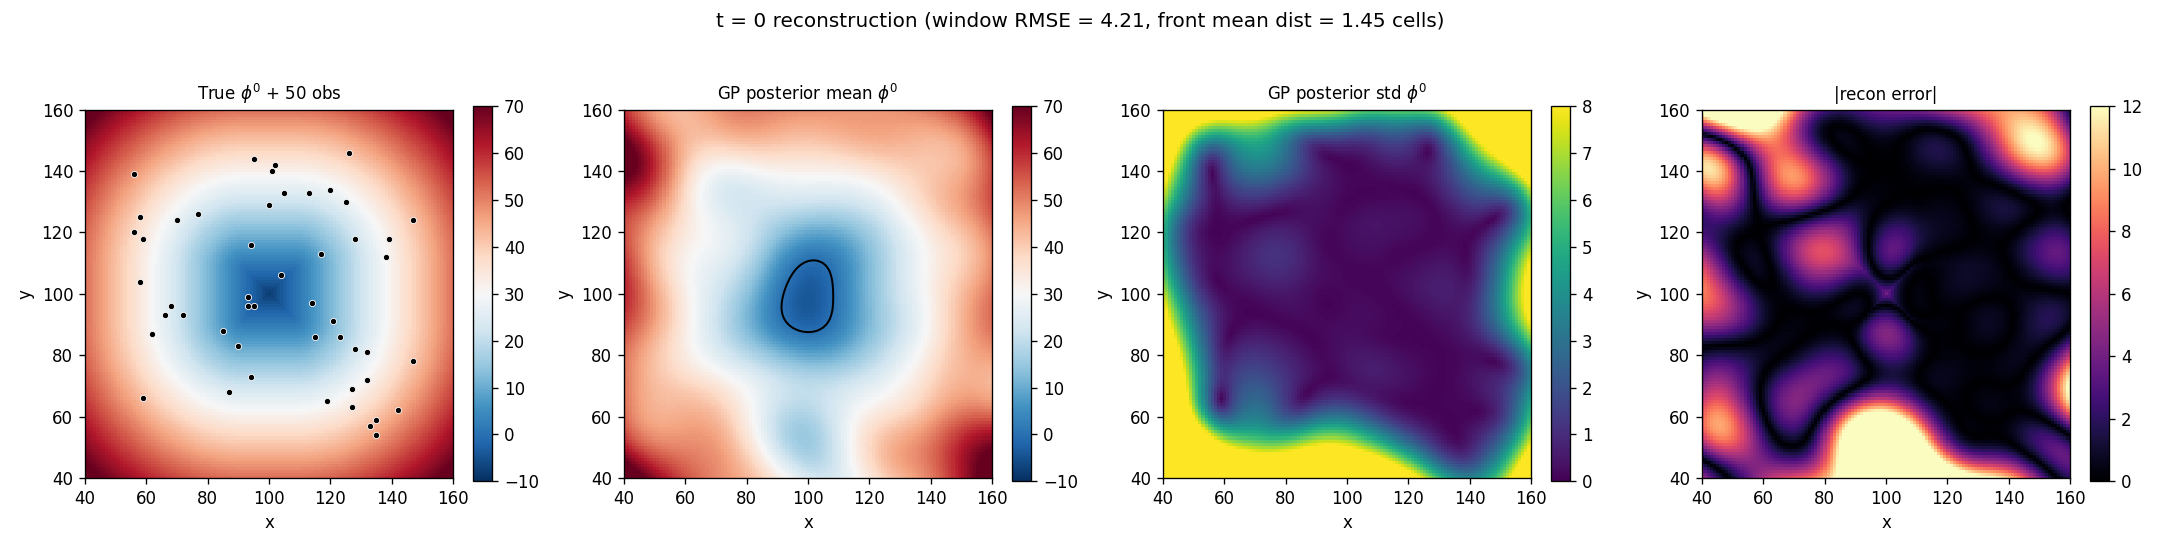
\includegraphics[width=\linewidth]{t0_reconstruction.png}
  \caption{$t=0$. True $\phi^{0}$ with the 50 sampled observations (black), GP
    posterior mean (note the rounded reconstruction of the sharp square front),
    posterior std (low where observed, high at unobserved corners), and
    $|$reconstruction error$|$.}
  \label{fig:t0}
\end{figure}

\begin{figure}[h]
  \centering
  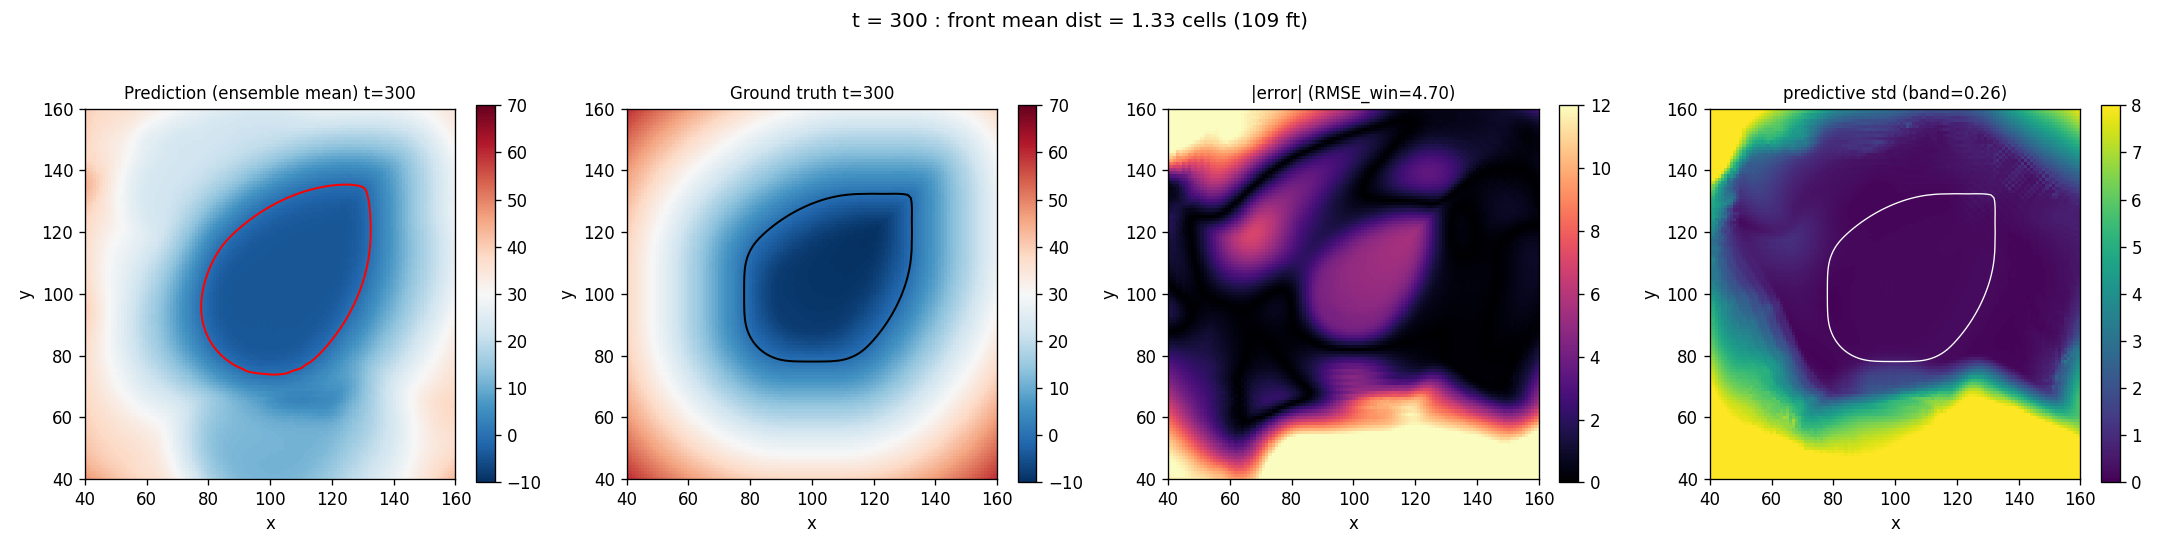
\includegraphics[width=\linewidth]{comparison_t300.png}
  \caption{$t=300$. Prediction (ensemble mean, red contour) vs.\ ground truth
    (black), absolute error, and predictive std with the GT front overlaid
    (white). Fronts agree to $1.33$ cells mean; shape differences persist at the
    wind-driven tip.}
  \label{fig:t300}
\end{figure}

\begin{figure}[h]
  \centering
  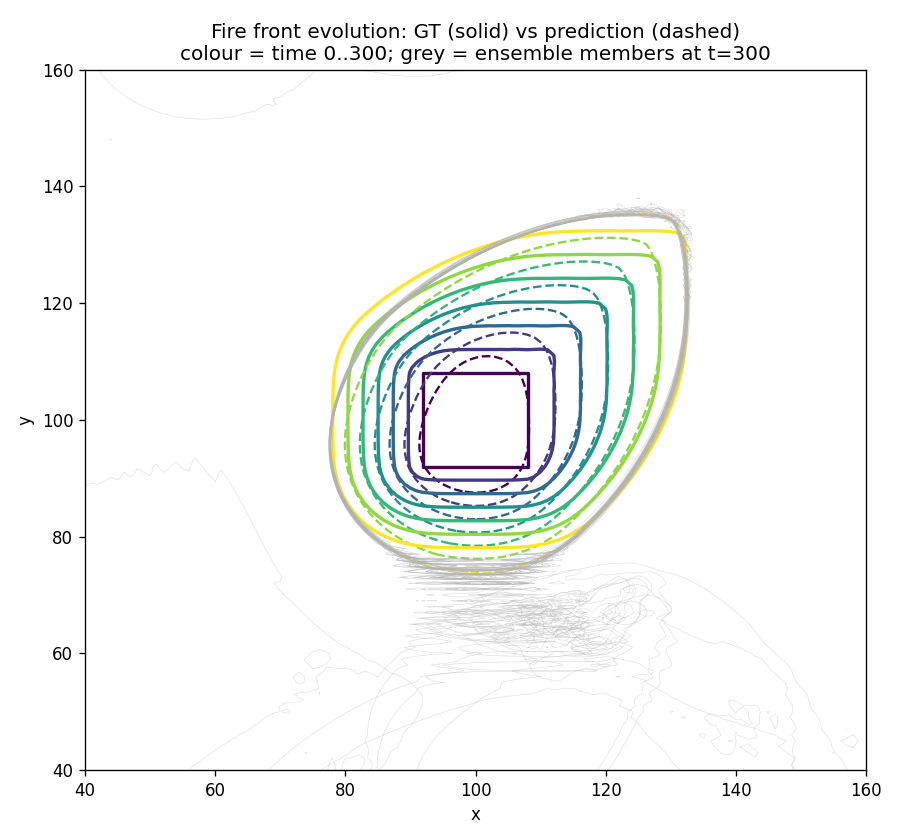
\includegraphics[width=0.62\linewidth]{front_evolution.png}
  \caption{Fire-front evolution, GT (solid) vs.\ prediction (dashed), colour-coded
    in time $0\to300$. The $t=0$ GT front is the sharp square; the prediction
    starts rounded yet tracks the teardrop spread. Grey curves are 40 ensemble
    members at $t=300$ (uncertainty band).}
  \label{fig:front}
\end{figure}

\begin{figure}[h]
  \centering
  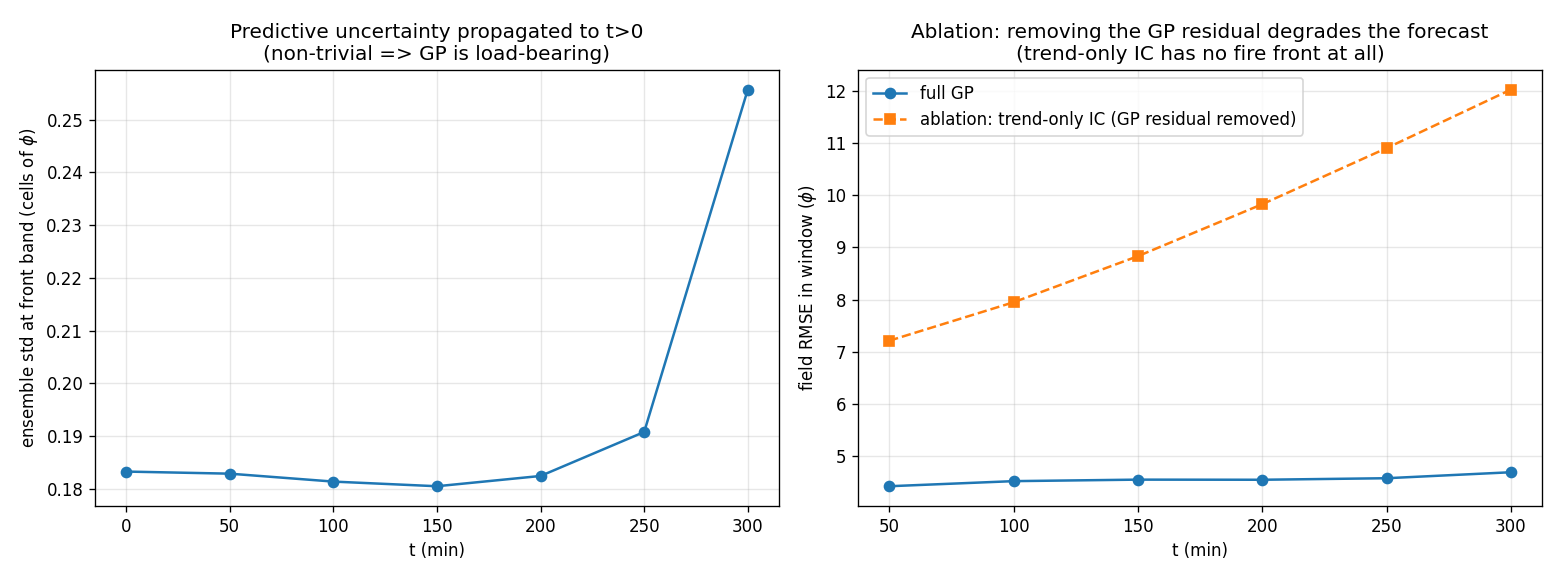
\includegraphics[width=\linewidth]{diagnostics.png}
  \caption{Load-bearing diagnostics. Left: front-band ensemble std grows with
    time (uncertainty propagated, not collapsed). Right: ablation --- removing the
    GP residual (trend-only IC, which has no front) degrades window RMSE from
    $\approx4.5$ to $7$--$12$.}
  \label{fig:diag}
\end{figure}

\section{Sources}

\begin{itemize}\itemsep0pt
  \item M.~Raissi, P.~Perdikaris, G.~E.~Karniadakis, \emph{Numerical Gaussian
        Processes for Time-dependent and Non-linear Partial Differential
        Equations} --- joint multi-output GP / Euler-embedded kernel construction
        \eqref{eq:joint-gp}.
  \item R.~C.~Rothermel (1972), \emph{A Mathematical Model for Predicting Fire
        Spread} --- rate-of-spread \eqref{eq:Rf}--\eqref{eq:windfactor}
        (\texttt{gp/docs/}).
  \item D.~Mu\~noz-Esparza et al.\ (2018), \emph{An Accurate Fire-Spread Algorithm
        in the WRF Model Using the Level-Set Method} --- level-set form
        \eqref{eq:levelset} (\texttt{gp/docs/}).
  \item \texttt{simulation.ipynb} --- source of truth for constants, operators,
        and ground truth; \texttt{gp/UNITS.md} --- units ($\Delta t=1$ min,
        $\Delta x=82.021$ ft).
\end{itemize}

\section{Notes}

\begin{itemize}\itemsep0pt
  \item \textbf{Worked:} sparse central inference + identical physics gives a
        front tracked to $\sim1.4$ cells; the level-set speed $F=R_f$ is
        independent of $\lvert\nabla\phi\rvert$, so once the front is located it
        stays located (the slight front-distance \emph{decrease} over time is
        curvature/viscosity smoothing of the rounded prediction toward the GT).
  \item \textbf{Limitations:} (1) far-field reconstruction reverts to the
        quadratic trend (full-grid RMSE inflated; fire unaffected); (2) front-band
        predictive std is modest ($0.18$--$0.26$ cells) because 50 central
        observations strongly constrain the front; (3) the operator is identical
        by design, so this trial tests \emph{initial-state inference $+$ uncertainty
        propagation}, not operator learning.
  \item \textbf{Next-trial ideas:} replace the quadratic trend with a
        monotone-radial-basis far-field model; condition on fewer / noisier
        observations to enlarge predictive variance; add process noise $Q$
        from the Euler truncation; compare ensemble pushforward against the
        explicit linearised $K_n=J_{n-1}K_{n-1}J_{n-1}^{\!\top}$ propagation.
\end{itemize}

\end{document}
